% original cutmix table. I don't know how to increase it so using the version below for now. But this one looks better IMHO
% \begin{table}[h!]
%   \centering
%   \small
%   \tabcolsep=0.07cm
%   \begin{tabular}{@{}ccccc@{}}
%   & Original  &  Mixup \cite{zhang2017_mixup} & CutMix \cite{yun2019_cutmix}\\
%   \multirow{4}{*}{Image} &  \multirow{4}{*}{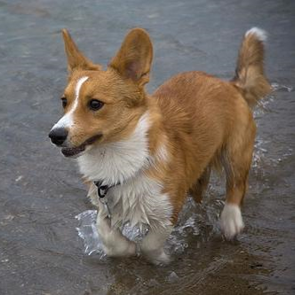
\includegraphics[width=0.10\linewidth]{images/dog.png}}
%   &  \multirow{4}{*}{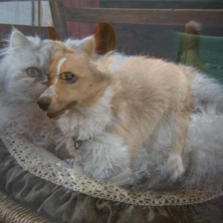
\includegraphics[width=0.10\linewidth]{images/dog_mixup.png}}
%   &  \multirow{4}{*}{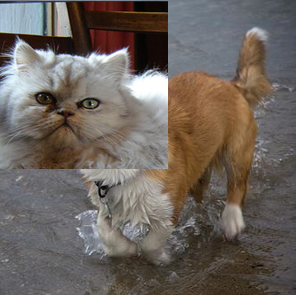
\includegraphics[width=0.10\linewidth]{images/dog_cutmix.png}} \\ 
%   & & & \\ 
%   & & & \\
%   & & & \\ \midrule
%   %
%   \multirow{2}{*}{Label} 
%   &\multirow{2}{*}{Dog 1.0}
%   &\multirow{2}{*}{\begin{tabular}[c]{@{}c@{}}Dog 0.5\\ Cat 0.5\end{tabular}}
%   &\multirow{2}{*}{\begin{tabular}[c]{@{}c@{}}Dog 0.6\\ Cat 0.4\end{tabular}} \\ 
%     & & & \\  \toprule

%   \end{tabular}
%   \caption{Example of Mixup/CutMix augmentations}
%   \label{tab:cutmix}
%   \end{table}


  \begin{figure}[h!]
    \centering
    \subfloat[][Original \\ Dog 1.0]{
      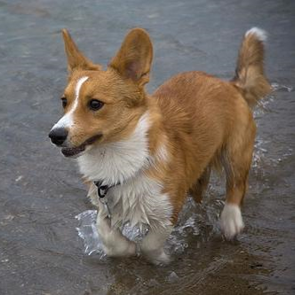
\includegraphics[scale=.55]{images/dog.png}
    }\hfill%
    \subfloat[][Mixup \\ Dog 0.5 Cat 0.5]{
      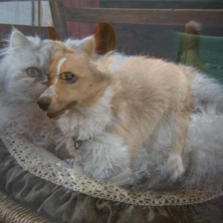
\includegraphics[scale=.55]{images/dog_mixup.png}
    }\hfill%
    \subfloat[][Cutmix \\ Dog 0.6 Cat 0.4]{
      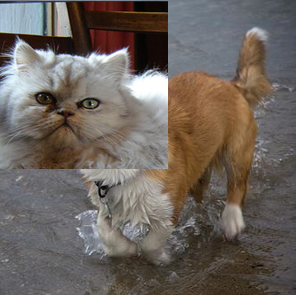
\includegraphics[scale=.55]{images/dog_cutmix.png}
    }
    \caption{Example of Mixup/CutMix augmentations. Label for each image during training is shown in sub-captions.}
    \label{fig:cutmix}

  \end{figure}